\chapter{Mise en Oeuvre du Systeme}

\section{Pipeline NLP -- Embedding et Indexation}

\subsection{Segmentation en Articles (Chunking)}

La strategie de segmentation retenue est le \textbf{decoupage par article juridique}. Chaque article constitue une unite de sens autonome dans les textes de loi marocains. Cette approche presente trois avantages :

\begin{enumerate}
    \item \textbf{Integrite semantique} : Un article forme un enonce juridique complet.
    \item \textbf{Tracabilite} : La citation dans les reponses generees renvoie a l'article exact.
    \item \textbf{Metadonnees riches} : Chaque chunk herite du contexte hierarchique (chapitre, section, livre).
\end{enumerate}

La comparaison des approches de chunking est synthetisee dans le Tableau~\ref{tab:chunking-strategies} :

\begin{table}[h]
\centering
\renewcommand{\arraystretch}{1.3}
\begin{tabular}{|l|p{4cm}|p{4cm}|}
\hline
\rowcolor{LightBlue}
\textbf{\color{PrimaryBlue}Approche} & \textbf{\color{PrimaryBlue}Avantage} & \textbf{\color{PrimaryBlue}Inconvenient} \\
\hline
Par article (retenue) & Precision juridique, tracabilite & Articles tres longs (rares) \\
Fenetre fixe (512 tokens) & Uniformite & Casse les articles en deux \\
Fenetre glissante & Contexte continu & Duplication, bruit \\
\hline
\end{tabular}
\caption{Comparaison des strategies de chunking pour les textes juridiques}
\label{tab:chunking-strategies}
\end{table}

\subsection{Service d'Embedding}

Le pipeline d'embedding transforme chaque article arabe en un vecteur semantique de 1024 dimensions via le modele \texttt{intfloat/multilingual-e5-large} (560M parametres). L'architecture du service est presentee dans la Figure~\ref{fig:embedding-service} :

\begin{figure}[H]
    \centering
    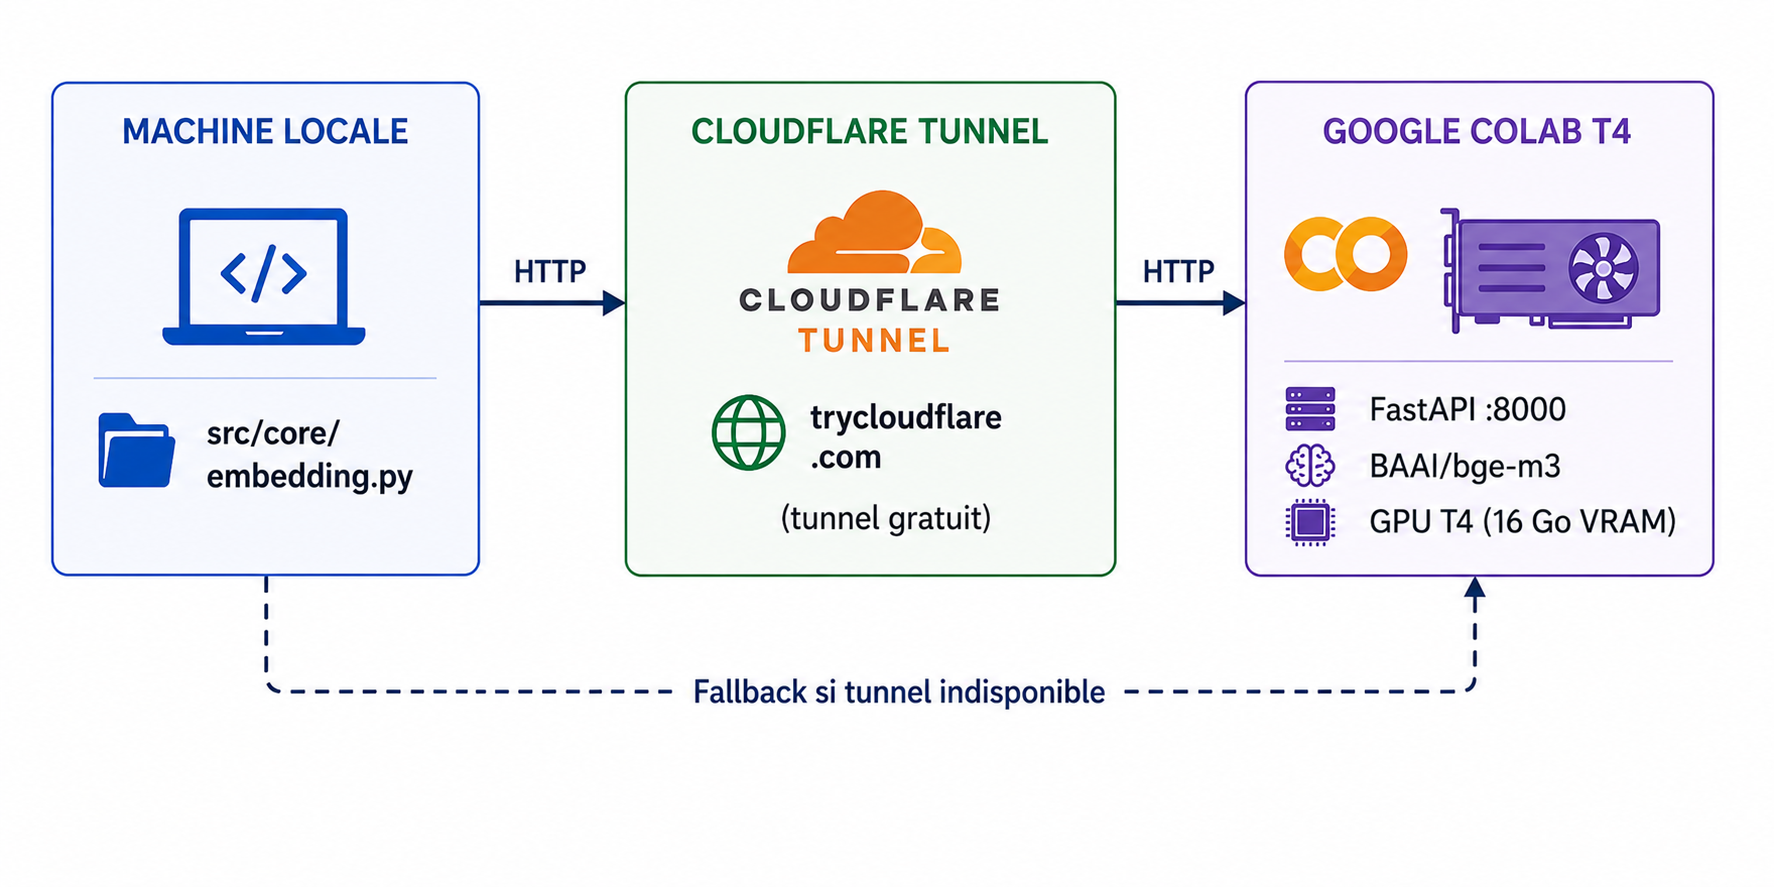
\includegraphics[width=0.9\textwidth]{images/illustrations/embedding_service_architecture.png}
    \caption{Remote embedding service architecture }
    \label{fig:embedding-service}
\end{figure}

Le service expose un endpoint \texttt{POST /embed} qui accepte une liste de textes arabes et retourne leurs vecteurs. En cas d'indisponibilite du tunnel (GPU Colab deconnecte), le systeme bascule automatiquement sur un embedding CPU local avec le modele E5-base (768 dimensions, 278M parametres), assurant la continuite de service.

Le Tableau~\ref{tab:embedding-models} resume les performances des 5 modeles d'embedding evalues lors de notre benchmark multilingue. Le modele \textbf{BGE-M3} arrive en tete sur l'ensemble des metriques globales.

\begin{table}[h]
\centering
\renewcommand{\arraystretch}{1.3}
\begin{tabular}{|l|r|r|r|r|r|r|}
\hline
\rowcolor{LightBlue}
\textbf{\color{PrimaryBlue}Modèle} &
\textbf{\color{PrimaryBlue}Dim.} &
\textbf{\color{PrimaryBlue}Params} &
\textbf{\color{PrimaryBlue}P@1} &
\textbf{\color{PrimaryBlue}P@5} &
\textbf{\color{PrimaryBlue}MRR} &
\textbf{\color{PrimaryBlue}NDCG} \\
\hline
BGE-M3 & 1024 & 568M & 0.85 & 0.20 & 0.92 & 0.94 \\
E5-large (multilingual) & 1024 & 560M & 0.80 & 0.20 & 0.89 & 0.91 \\
LaBSE & 768 & 470M & 0.70 & 0.18 & 0.80 & 0.82 \\
E5-base (multilingual) & 768 & 278M & 0.59 & 0.19 & 0.76 & 0.80 \\
MPNet (multilingual) & 768 & 278M & 0.54 & 0.19 & 0.71 & 0.77 \\
\hline
\end{tabular}
\caption{Classement global des modèles d'embedding sur le corpus juridique marocain (toutes langues)}
\label{tab:embedding-models}
\end{table}
BGE-M3 domine le benchmark avec un P@1 de 0.85 et un MRR de 0.92, et se montre particulierement performant pour les requetes en arabe formel (P@1 = 0.92). Le modele E5-large, bien que legerement en retrait sur les metriques globales, reste le modele utilise dans le pipeline actuel en raison de sa disponibilite immediate au format GGUF et de la coherence de la famille E5 qui facilite le fallback CPU vers E5-base. Une migration vers BGE-M3 est envisagee pour les versions futures du systeme.

\subsection{Debit d'Indexation}

Le Tableau~\ref{tab:indexation-debit} presente le debit d'indexation mesure selon le mode d'embedding :

\begin{table}[h]
\centering
\renewcommand{\arraystretch}{1.3}
\begin{tabular}{|l|r|r|}
\hline
\rowcolor{LightBlue}
\textbf{\color{PrimaryBlue}Mode} & \textbf{\color{PrimaryBlue}Articles/s} & \textbf{\color{PrimaryBlue}Latence/article} \\
\hline
GPU Colab T4 (E5-large, tunnel) & $\sim$20 & $\sim$50 ms \\
CPU local (E5-base) & $\sim$3 & $\sim$300 ms \\
\hline
\end{tabular}
\caption{Debit d'indexation selon le mode d'embedding}
\label{tab:indexation-debit}
\end{table}

\section{Strategies de Recherche}

\subsection{Architecture de la Recherche Hybride}

Le moteur de recherche implemente trois strategies via un pattern Factory (Listing~\ref{lst:retrieval-factory}) :

\begin{verbatim}
from src.retrieval.strategies.dense import DenseRetrieval
from src.retrieval.strategies.bm25 import BM25Retrieval
from src.retrieval.strategies.rrf import RRFRetrieval

def create_retrieval_strategy(name: str, **kwargs):
    if name == "dense":
        return DenseRetrieval()
    elif name == "bm25":
        return BM25Retrieval()
    elif name == "rrf":
        return RRFRetrieval(k_rrf=kwargs.get("k_rrf", 60))
\end{verbatim}
\label{lst:retrieval-factory}

\subsection{Recherche Dense (DenseRetrieval)}

La recherche dense exploite l'index HNSW de pgvector pour la similarite cosinus. Le processus est le suivant :

\begin{enumerate}
    \item La requete utilisateur est encodee en vecteur 1024d par le service d'embedding.
    \item pgvector execute une recherche par similarite cosinus avec l'operateur \texttt{<=>}.
    \item Les K articles les plus similaires sont retournes avec leur score de similarite.
\end{enumerate}

L'implementation utilise une connexion a la base de donnees via \texttt{src/db/session.py} et l'embedder via \texttt{src/core/embedding.py}. L'index HNSW garantit une latence de recherche inferieure a 5 ms pour $\sim$2\,400 vecteurs.

\subsection{Recherche Lexicale BM25 (BM25Retrieval)}

Suite a l'echec du full-text search PostgreSQL pour l'arabe (0 resultat sur 32 requetes de test, cf. Section~\ref{sec:resultats}), la recherche BM25 a ete reimplementee avec le tokenizer arabe specialise developpe dans ce projet (\texttt{src/retrieval/strategies/arabic\_tokenizer.py}). Le processus est le suivant :

\begin{enumerate}
    \item \textbf{Chargement} : Tous les documents actifs sont charges en memoire au premier appel (\textit{lazy loading}).
    \item \textbf{Tokenisation} : Chaque document est normalise (ArabicNormalizer) puis tokenise avec extraction par regex Unicode, suppression des 60+ stop words juridiques, et filtrage des tokens courts ($\ge 2$ caracteres).
    \item \textbf{Indexation} : Un index BM25Okapi (rank-bm25) est construit sur les documents tokenises.
    \item \textbf{Recherche} : La requete est tokenisee avec le meme pipeline, les scores BM25 sont calcules pour tous les documents, et les K meilleurs sont retournes.
\end{enumerate}

Le Tableau~\ref{tab:bm25-tokenization} illustre l'effet de la tokenisation arabe sur un exemple de texte juridique :

\begin{table}[h]
\centering
\renewcommand{\arraystretch}{1.3}
\begin{tabular}{|p{6cm}|p{6cm}|}
\hline
\rowcolor{LightBlue}
\textbf{\color{PrimaryBlue}Texte original} & \textbf{\color{PrimaryBlue}Tokens apres normalisation} \\
\hline
\textarabic{المادة 513 من القانون الجنائي المغربي تنص على انه يعتبر الحدث البالغ من العمر اقل من 16 سنة في وضعية صعبة} & \texttt{[\textarabic{الجنائي}, \textarabic{المغربي}, \textarabic{تنص}, \textarabic{انه}, \textarabic{يعتبر}, \textarabic{الحدث}, \textarabic{البالغ}, \textarabic{العمر}, \textarabic{اقل}, \textarabic{سنة}, \textarabic{وضعية}, \textarabic{صعبة}]} \\
\hline
\end{tabular}
\caption{Exemple de tokenisation arabe avec stop words et filtrage}
\label{tab:bm25-tokenization}
\end{table}

\subsection{Fusion RRF (RRFRetrieval)}

La fusion RRF (Reciprocal Rank Fusion) combine les classements dense et lexical sans parametre a regler. La formule est la suivante :

\begin{equation}
\text{RRF}(d) = \frac{1}{k + \text{rank}_{\text{dense}}(d)} + \frac{1}{k + \text{rank}_{\text{bm25}}(d)}
\label{eq:rrf}
\end{equation}

ou $k = 60$ (constante de lissage) et $d$ designe un document (article juridique). Les deux canaux produisent chacun un classement top-20. Les rangs sont fusionnes par la formule~\ref{eq:rrf}, et les K meilleurs documents sont selectionnes pour la generation.

La Figure~\ref{fig:rrf-fusion} illustre le processus de fusion :
\begin{figure}[H]
    \centering
    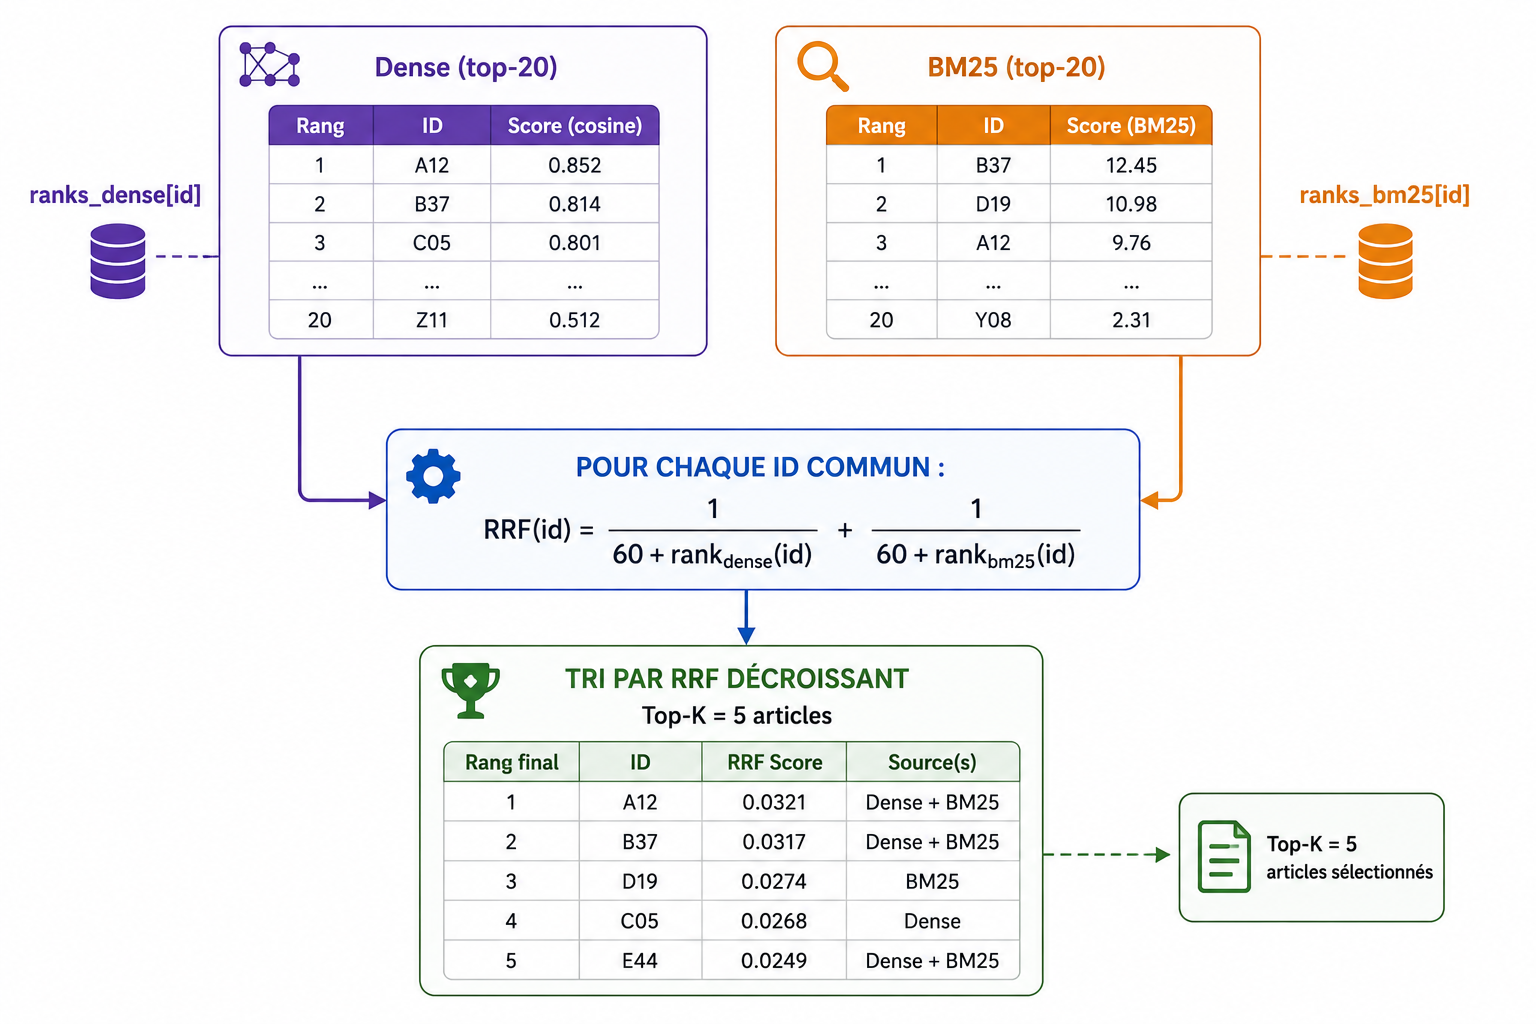
\includegraphics[width=0.9\textwidth]{images/illustrations/rrf_fusion_process.png}
    \caption{Reciprocal Rank Fusion}
    \label{fig:rrf-fusion}
\end{figure}

\section{Generation de Reponses Juridiques}

\subsection{Modele de Langage}

Le systeme utilise \textbf{Gemma 4 2B} (Google, 2025), un modele de langage de 2 milliards de parametres, quantifie en precision Q4\_K\_XL au format GGUF. Le Tableau~\ref{tab:llm-config} resume la configuration d'inference :

\begin{table}[h]
\centering
\renewcommand{\arraystretch}{1.3}
\begin{tabular}{|l|l|}
\hline
\rowcolor{LightBlue}
\textbf{\color{PrimaryBlue}Parametre} & \textbf{\color{PrimaryBlue}Valeur} \\
\hline
Modele & Google Gemma 4 2B instruct \\
Quantification & Q4\_K\_XL (GGUF) \\
Taille sur disque & $\sim$1.1 Go (reduction 73\% vs FP16) \\
Moteur d'inference & llama.cpp \\
GPU Layers & -1 (tous sur GPU si disponible) \\
Contexte maximal & 16\,384 tokens \\
Temperature & 0.3 \\
Top-P & 0.9 \\
Max tokens generes & 512 \\
\hline
\end{tabular}
\caption{Configuration du LLM pour la generation de reponses juridiques}
\label{tab:llm-config}
\end{table}

\subsection{Construction du Prompt}

Le prompt est construit en trois parties (Listing~\ref{lst:prompt-template}) :

\begin{enumerate}
    \item \textbf{Instruction systeme} : Definition du role d'assistant juridique marocain, contrainte de fidelite au contexte, langue de reponse (arabe uniquement).
    \item \textbf{Contexte} : Les K articles retrouves formates avec leur reference (\textarabic{المادة} $X$ \textarabic{من} $Loi$).
    \item \textbf{Question} : La requete originale de l'utilisateur.
\end{enumerate}

\begin{jsonblock}{Prompt Template (Arabe)}
Tu es un assistant juridique specialise dans le droit marocain.
Tu reponds UNIQUEMENT en arabe.
Base ta reponse EXCLUSIVEMENT sur les articles de loi fournis.
N'invente JAMAIS d'article de loi.
Cite TOUJOURS les numeros d'article utilises.

\textarabic{النصوص القانونية المسترجعة:}

[1] \textarabic{المادة 513 من code penal maroc ar:}
\textarabic{يعتبر الحدث البالغ من العمر اقل من 16 سنة...}

[2] \textarabic{المادة 508 من code penal maroc ar:}
\textarabic{يعاقب على السرقة الموصوفة بالسجن...}

\textarabic{بناء على النصوص القانونية اعلاه فقط، اجب على السؤال التالي:}
\textarabic{ما هي عقوبة السرقة في القانون المغربي؟}
\end{jsonblock}
\label{lst:prompt-template}

\subsection{Format de la Reponse}

La reponse generee suit une structure en quatre parties (Tableau~\ref{tab:response-format}) :

\begin{table}[h]
\centering
\renewcommand{\arraystretch}{1.3}
\begin{tabular}{|l|p{6cm}|l|}
\hline
\rowcolor{LightBlue}
\textbf{\color{PrimaryBlue}Section} & \textbf{\color{PrimaryBlue}Contenu} & \textbf{\color{PrimaryBlue}Exemple} \\
\hline
1. Resume & Synthese de la reponse en une phrase & \textarabic{حسب المادتين 508 و 509...} \\
2. Analyse & Developpement juridique detaille & \textarabic{تنص المادة 508 على انه...} \\
3. Verdict & Conclusion juridique fondee & \textarabic{وبالتالي فان عقوبة السرقة...} \\
4. Sources & Liste des articles cites & \textarabic{المادة 508، المادة 509} \\
\hline
\end{tabular}
\caption{Structure de la reponse juridique generee par le LLM}
\label{tab:response-format}
\end{table}

\subsection{Enrichissement Contextuel}

Le LLM enrichit la reponse au-dela de la simple restitution des articles. Cet enrichissement contextuel -- synthese multi-sources, references croisees, formulation de verdicts -- est un comportement \textbf{souhaite et ancre} dans les documents retrouves. Il se distingue de l'hallucination car chaque affirmation derive d'un article source identifiable. Le Tableau~\ref{tab:enrichment-vs-hallucination} clarifie cette distinction :

\begin{table}[h]
\centering
\renewcommand{\arraystretch}{1.3}
\begin{tabular}{|p{4cm}|p{4cm}|p{4cm}|}
\hline
\rowcolor{LightBlue}
\textbf{\color{PrimaryBlue}Comportement} & \textbf{\color{PrimaryBlue}Exemple} & \textbf{\color{PrimaryBlue}Classification} \\
\hline
Synthese multi-articles & \textarabic{حسب المادتين 508 و 509، يعاقب...} & \textbf{Enrichissement} (ancre) \\
Citation d'article & \textarabic{طبقا للمادة 513 من القانون الجنائي} & \textbf{Enrichissement} (ancre) \\
Conclusion juridique & \textarabic{وبالتالي فان الفعل يعتبر جريمة...} & \textbf{Enrichissement} (ancre) \\
Invention d'article inexistant & \textarabic{المادة 999 تنص على...} (n'existe pas) & \textbf{Hallucination} (non ancre) \\
Contradiction avec la loi & Reponse contraire au texte source & \textbf{Hallucination} (non ancre) \\
\hline
\end{tabular}
\caption{Distinction entre enrichissement contextuel legitime et hallucination}
\label{tab:enrichment-vs-hallucination}
\end{table}

\section{API REST (FastAPI)}

\subsection{Endpoints}

L'API expose six endpoints principaux (Tableau~\ref{tab:api-endpoints}) :

\begin{table}[h]
\centering
\renewcommand{\arraystretch}{1.3}
\begin{tabular}{|l|l|l|}
\hline
\rowcolor{LightBlue}
\textbf{\color{PrimaryBlue}Methode} & \textbf{\color{PrimaryBlue}Endpoint} & \textbf{\color{PrimaryBlue}Description} \\
\hline
GET & \texttt{/api/v1/health} & Etat du systeme et des services \\
POST & \texttt{/api/v1/search} & Recherche juridique (retrieval seul) \\
POST & \texttt{/api/v1/ask} & Question-reponse juridique (RAG complet) \\
GET & \texttt{/api/v1/laws} & Liste des lois indexees \\
POST & \texttt{/api/v1/upload} & Upload de nouveaux PDF juridiques \\
GET & \texttt{/api/v1/conversations} & Historique des conversations \\
\hline
\end{tabular}
\caption{Endpoints de l'API FastAPI}
\label{tab:api-endpoints}
\end{table}

\subsection{Format Requete/Reponse -- /ask}

L'endpoint principal \texttt{/api/v1/ask} accepte le format de requete suivant :

\begin{jsonblock}{Requete JSON /api/v1/ask}
POST /api/v1/ask
{
  "query": "\textarabic{ما هي عقوبة السرقة في القانون المغربي؟}",
  "domain": "criminal",
  "top_k": 5,
  "strategy": "rrf"
}
\end{jsonblock}

Et retourne la reponse structuree du Listing~\ref{lst:ask-response} :

\begin{jsonblock}{Reponse JSON de l'API /ask}
\{\\
\quad "query": "\textarabic{ما هي عقوبة السرقة في القانون المغربي؟}",\\
\quad "short\_answer": "\textarabic{حسب المادتين 508 و 509 من القانون الجنائي...}",\\
\quad "long\_answer": "\textarabic{تنص المادة 508 على انه يعاقب على السرقة...}",\\
\quad "sources": [\\
\qquad \{\\
\qquad\quad "article\_number": "508",\\
\qquad\quad "law\_name": "code penal maroc ar",\\
\qquad\quad "domain": "criminal",\\
\qquad\quad "relevance\_score": 0.92\\
\qquad \}\\
\quad ],\\
\quad "disclaimer": "\textarabic{هذه الاجابة مولدة اليا...}",\\
\quad "session\_id": "uuid-v4",\\
\quad "search\_time\_ms": 12.5,\\
\quad "generation\_time\_ms": 2340.0,\\
\quad "total\_time\_ms": 2352.5,\\
\quad "model\_name": "Gemma 4 2B"\\
\}
\end{jsonblock}
\label{lst:ask-response}

\section{Interfaces Utilisateur}

\subsection{Interface Web (SvelteKit)}

L'interface web est developpee avec SvelteKit 5, Tailwind CSS 4, et TypeScript 6 (Tableau~\ref{tab:frontend-stack}). Elle offre une experience de recherche juridique complete avec :

\begin{itemize}
    \item Barre de recherche avec selection du domaine juridique et de la strategie
    \item Affichage des articles retrouves avec score de pertinence
    \item Reponse generee formatee avec sections (resume, analyse, sources)
    \item Historique des conversations
    \item Upload de nouveaux documents PDF
\end{itemize}

\begin{table}[h]
\centering
\renewcommand{\arraystretch}{1.3}
\begin{tabular}{|l|l|}
\hline
\rowcolor{LightBlue}
\textbf{\color{PrimaryBlue}Technologie} & \textbf{\color{PrimaryBlue}Version / Role} \\
\hline
SvelteKit & 5 -- Framework frontend \\
Svelte & 5 -- Composants reactifs \\
Tailwind CSS & 4 -- Styling utilitaire \\
TypeScript & 6 -- Typage statique \\
Vite & 8 -- Bundler et serveur de developpement \\
Lucide Icons & 1 -- Iconographie \\
marked & 18 -- Rendu Markdown des reponses \\
DOMPurify & 3 -- Sanitization HTML \\
Playwright & 1.59 -- Tests end-to-end \\
\hline
\end{tabular}
\caption{Stack technique du frontend SvelteKit}
\label{tab:frontend-stack}
\end{table}

\subsection{Interface Terminal (TUI)}

Une interface terminal (TUI) developpee avec le framework Textual (Python) permet la gestion du corpus en ligne de commande :

\begin{itemize}
    \item Navigation par domaines juridiques (7 domaines)
    \item Visualisation des articles et metadonnees
    \item Recherche et exploration du corpus
    \item Upload de nouveaux documents
    \item Raccourcis clavier pour la navigation rapide
\end{itemize}

\subsection{Scripts CLI}

Un ensemble de scripts en ligne de commande complete les interfaces (Tableau~\ref{tab:cli-scripts}) :

\begin{table}[h]
\centering
\renewcommand{\arraystretch}{1.3}
\begin{tabular}{|l|p{7cm}|}
\hline
\rowcolor{LightBlue}
\textbf{\color{PrimaryBlue}Script} & \textbf{\color{PrimaryBlue}Fonction} \\
\hline
\texttt{embed\_all\_articles.py} & Indexation complete du corpus par lots \\
\texttt{batch\_process\_pdfs.py} & Traitement par lots de PDF \\
\texttt{run\_preprocessing\_pipeline.py} & Pipeline complet de preprocessing \\
\texttt{seed\_test\_data.py} & Peuplement de la base de test \\
\texttt{check\_retrieval\_quality.py} & Verification de la qualite du retrieval \\
\texttt{parse\_legal\_structure.py} & Parsing de la structure des lois \\
\hline
\end{tabular}
\caption{Scripts CLI principaux}
\label{tab:cli-scripts}
\end{table}

\section{Deploiement et Infrastructure}

\subsection{Conteneurisation Docker}

L'infrastructure est entierement conteneurisee via Docker Compose (cf. Listing~\ref{lst:docker-compose}, Section~\ref{sec:conception-docker}). Les services deployes sont :

\begin{itemize}
    \item \textbf{legal-rag-postgres} : PostgreSQL 16 + pgvector 0.7.4 (image custom)
    \item \textbf{pgadmin} : Interface d'administration PostgreSQL (port 5050)
    \item \textbf{api} : API FastAPI (port 8000, image custom)
    \item \textbf{web} : Frontend SvelteKit (port 5173, image custom)
\end{itemize}

\subsection{Services Distants}

Deux services sont heberges sur Google Colab (GPU T4 gratuit) et exposes via Cloudflare Tunnel :

\begin{itemize}
    \item \textbf{Service d'embedding} : E5-large sur GPU T4, endpoint \texttt{/embed}, latence $\sim$50 ms/texte.
    \item \textbf{Service LLM} : Gemma 4 2B Q4\_K\_XL via llama.cpp, endpoint \texttt{/generate}, latence $\sim$2-5 s/reponse.
\end{itemize}

Le Tableau~\ref{tab:latency-breakdown} detaille la latence de chaque composant du pipeline :

\begin{table}[h]
\centering
\renewcommand{\arraystretch}{1.3}
\begin{tabular}{|l|r|r|}
\hline
\rowcolor{LightBlue}
\textbf{\color{PrimaryBlue}Composant} & \textbf{\color{PrimaryBlue}Latence (ms)} & \textbf{\color{PrimaryBlue}\% du total} \\
\hline
Recherche pgvector (cosine) & $\sim$2 & 0.02\% \\
BM25 rank-bm25 (en memoire) & $\sim$5 & 0.04\% \\
Fusion RRF & $\sim$1 & 0.01\% \\
Embedding (tunnel Colab) & $\sim$5\,500 & 47\% \\
Construction du prompt & $\sim$1 & 0.01\% \\
Generation LLM (llama.cpp) & $\sim$6\,200 & 53\% \\
\hline
\textbf{Total pipeline} & \textbf{$\sim$11\,700} & \textbf{100\%} \\
\hline
\end{tabular}
\caption{Decomposition de la latence du pipeline RAG complet}
\label{tab:latency-breakdown}
\end{table}

Le goulot d'etranglement principal est le service d'embedding distant via Cloudflare Tunnel ($\sim$5.5 s). Un deploiement local de l'embedding (E5-base sur CPU) reduirait cette latence a $\sim$100 ms, divisant le temps total par 2.

\section{Conclusion de la Mise en Oeuvre}

La mise en oeuvre du systeme Moroccan Legal RAG a permis de concretiser l'architecture concue au Chapitre~3 en un systeme operationnel. Les points cles de l'implementation sont :

\begin{enumerate}
    \item \textbf{Embedding optimise} : Benchmark de 5 modeles, BGE-M3 en tete (P@1=0.85, MRR=0.92), pipeline actuel base sur E5-large avec fallback CPU E5-base. Une migration vers BGE-M3 est prevue.

    \item \textbf{Recherche hybride operationnelle} : Trois strategies (Dense, BM25 avec tokenizer arabe, RRF) via un pattern Factory. Le BM25 arabe corrige l'echec du FTS PostgreSQL.

    \item \textbf{Generation enrichie et ancre} : LLM Gemma 4 2B quantifie Q4\_K\_XL ($\sim$1.1 Go), prompt structure en trois parties, reponse en quatre sections. L'enrichissement contextuel (synthese, verdicts, references croisees) est distingue de l'hallucination.

    \item \textbf{API REST complete} : 6 endpoints documentes, format requete/reponse structure, historique des conversations.

    \item \textbf{Interfaces multiples} : Web (SvelteKit), terminal (Textual), et scripts CLI pour les traitements par lots.

    \item \textbf{Infrastructure legere} : Docker Compose, Cloudflare Tunnel, llama.cpp. Pipeline complet en $\sim$12 s par question, dont 53\% pour la generation LLM.
\end{enumerate}